\newpage
\thispagestyle{sectioned}
\chapter{Construyendo la idea: DemoCritics}

\section{Introducción}
Una vez que habíamos elegido la tecnología que soportaría el núcleo de nuestra aplicación, teníamos que decir que implementación le íbamos a dar a nuestra aplicación móvil. Para ello teníamos que tener en cuenta las características que nos ofrecía Wave:

Edición colaborativa.

Tiempo real.

Consistencia.

Después de darle unas cuantas vueltas de las posibles implementaciones que podríamos realizar sobre estas características potenciales, decidimos realizar una sesión de brain storming. En esta sesión aparecieron temas tan dispersos como wikis colaborativas, aplicaciones con inteligencia artificial, aportaciones colaborativas en política, edición de vídeos y música, cursos de formación colaborativos, etcétera.

\begin{figure}[H]
\centering
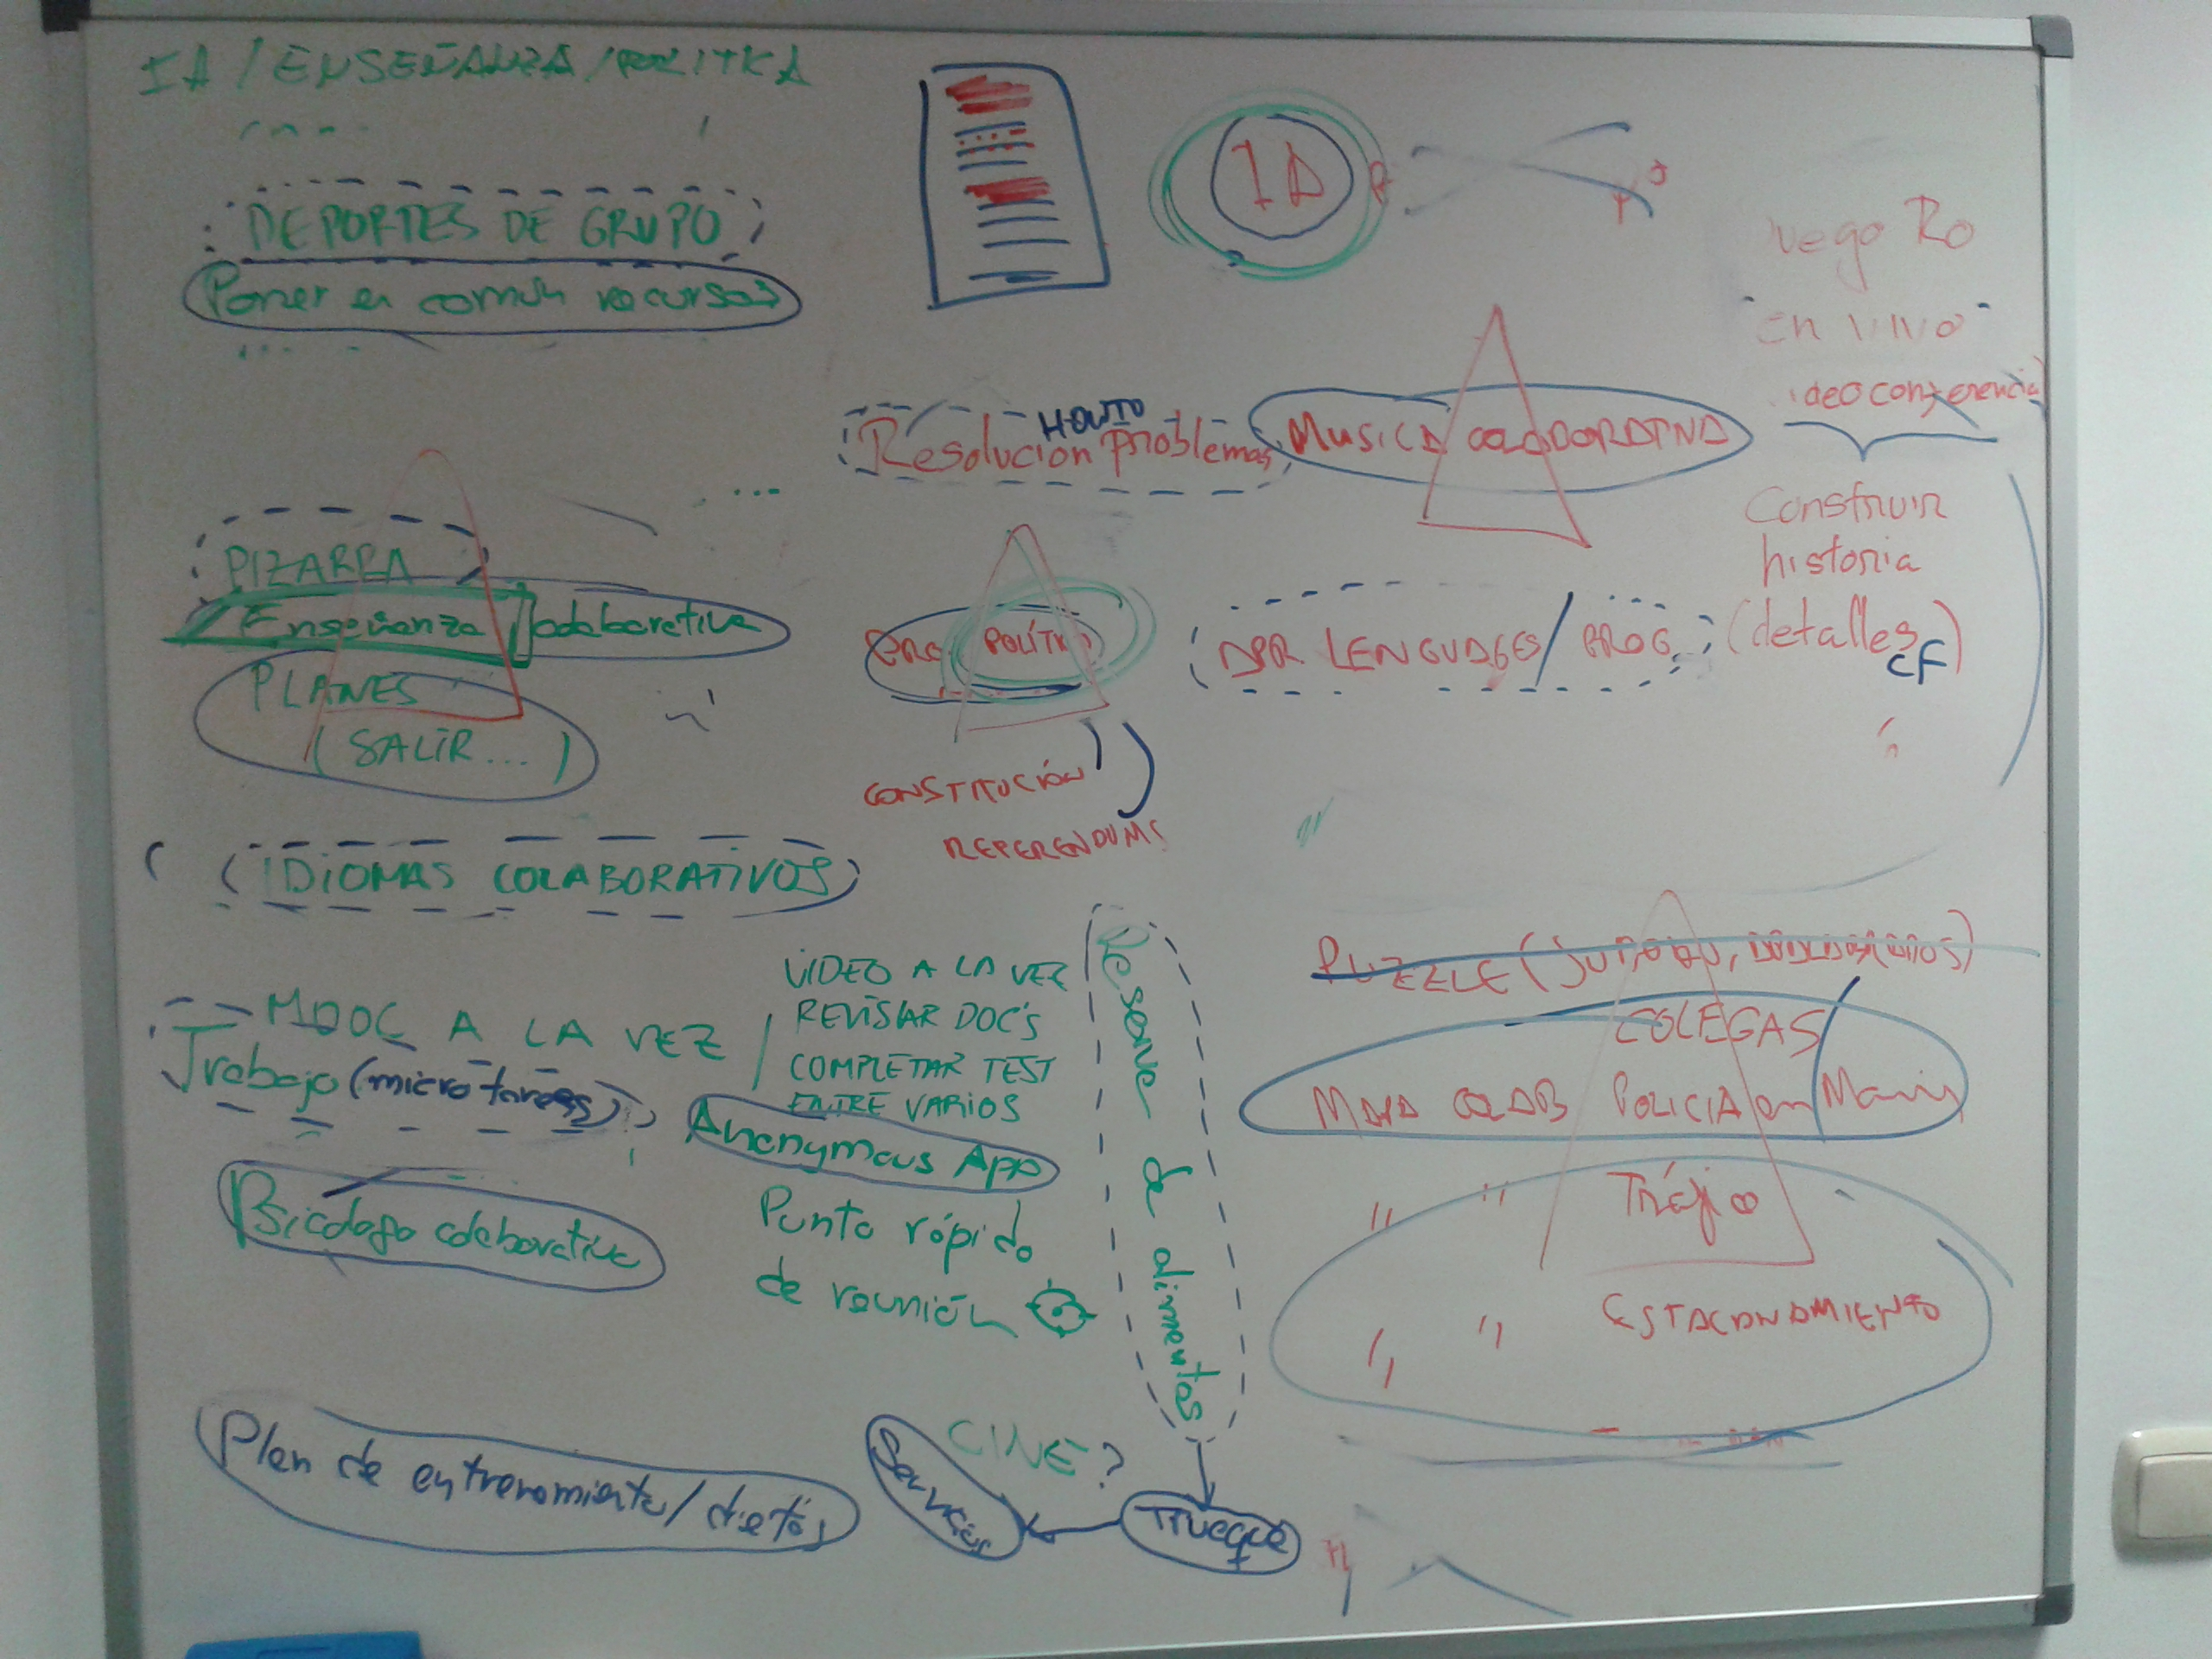
\includegraphics[keepaspectratio, scale=0.15]{Media/Captures/brainstorming.jpg}
\caption{Brainstorming sobre la idea a desarrollar}
\label{fig:brainstorming}
\end{figure}

Con un gran repertorio de ideas expuestas sobre la sesión, descartamos aquellas que no nos motivaban llevarlas a cabo. Por lo que nos quedamos con tres ideas fundamentales a desarrollar en nuestra aplicación: Política, Música, Inteligencia Artificial y Mapas. Surgieron varias ideas colaborativas como desarrollar documentos políticos, programas electorales, comunicación entre colectivos en tiempo real, aprendizaje de música, edición de partituras y obras, aplicaciones colaborativas con inteligencia artificial, edición de mapas en tiempo real, lexicalización, etcétera.

Finalmente debido a intereses comunes, decimos realizar una aplicación colaborativa relacionado con el mundo de la política. Con el objetivo de que pudiera tener cierta repercusión y utilidad en las próximas citas electorales durante el año 2015. En esta aplicación podríamos recurrir a la edición de contenidos en tiempo real, ya fueran propuestas políticas, programas electorales y otro tipo de documentos. Como también hacer uso de alguna herramienta de Inteligencia Artificial para automatizar algunas tareas o realizar recomendaciones sociales.

\subsection{Política en el mundo de la Informática}

A primera vista podemos pensar que la informática no parece entusiasmar a os informáticos. Pues podemos ubicar la política como una parte de las ciencias sociales, situando la informática en ciencias formales. Pero si factores como la gestión de los privilegios de una aplicación entre los que definiremos de alguna forma una jerarquía, estaremos haciendo política de alguna manera. También encontraremos características políticas en el diseño relacional de una base de datos. Definiendo los campos de una base de datos podemos encontraremos con algunos valores como el sexo, la nacionalidad, la edad o incluso las relaciones o restricciones que existen entre las tablas. Estaremos definiendo unas reglas básicas funcionamiento de la base de datos establecidas por unos principios políticos.

Además sumergiéndonos en el mundo de las licencias de uso en el desarrollo de software encontraremos más política aún. Licencias que determinan el uso de un tipo de software, ya sea para compartir, vender, distribuir copias, entre otros. Multitud de reglas políticas definidas en una licencia de uso. Así como las restricciones que establecemos en la metodología orientada a objetos, estableciendo las relaciones de herencia, restricción de métodos, variables, etcétera.

Regresando a la actualidad y basándonos en no muy lejanos acontecimientos pasados, habremos oído cómo algunos gobiernos recopilan datos de la actividad de los usuarios en las redes sociales, analizando todo el contenido que generan. Incluso vemos cómo algunas aplicaciones móviles piden aprobar permisos con los que operar libremente en tu dispositivo.

Como podemos observar la política está más integrada en la informática de lo que parece, dejando a un lado la informática más científica, más formal, pasando a la informática social, la de los gobiernos, la de los negocios o la de las relaciones sociales.

\subsection{Democracia}

\subsubsection{Democracia representativa}

\subsubsection{Democracia participativa}

\subsubsection{Democracia directa}

\subsubsection{Democracia deliberativa}


\subsection{Adentrándonos en la idea}
La idea a desarrollar generada en una época dónde la política parecía haber despertado el interés de una parte considerable de la ciudadanía, podría ser una herramienta útil para participar en temas políticos que forma sencilla y atractiva. Dejando atrás los tópicos yo no entiendo de política, la política es aburrida, no sé a quién votar o no he leído nunca un programa electoral entre otros.

La herramienta ofrecería una nueva forma de participar en la política y de llevar a los ciudadanos los programas electorales ofertados por las diferentes formaciones políticas. De tal forma que los ciudadanos pudieran leer aquellos puntos de los programas más leídos, debatidos, comentados, etcétera. Así cualquier usuario tendría todos programas electorales en su bolsillo, por lo que no tendría que ir a la página web de cada formación política y descargarse un documento de 200 páginas. Pensamos que esta forma de presentar un programa político en un mundo donde las posibilidades de  comunicarnos se han desarrollado exponencialmente, no era la mejor manera de llegar a la mayor parte de la ciudadanía.

Por otra parte, la aplicación también debería ofrecer alguna herramienta donde realizar propuestas y debatirlas entre todos. De tal forma que tanto la ciudadanía como las formaciones políticas pudieran saber en cualquier momento cuáles son las principales preocupaciones de los ciudadanos y qué medidas o soluciones proponen para resolverlas.

Desde un primer punto de vista subjetivo, la aplicación quedó dividida en dos partes. Por un lado tendríamos los programas políticos que presentaran las formaciones políticas. Y por otro, todas las propuestas que elaboraran los ciudadanos individualmente o en colectivos sociales.

\section{Estado del Arte}

En esta sección exploraremos las principales aplicaciones informáticas destinadas a la participación ciudadana en propuestas, lectura de programas electorales o divulgación de candidaturas.

\subsection{Programas Políticos}

En la actualidad no existe ningún tipo de aplicación orientada a debatir los programas electorales de los partidos políticos. Concretamente no hay ningún tipo de plataforma que agrupe los programas electorales de las diferentes candidaturas.
Lo más parecido que hemos podido encontrar han sido aplicaciones elaboradas por un partido político, orientada a dar a conocer su candidatura. En ella podremos ver la candidatura, vídeos y el programa electoral entre otros. Por ello pasamos a analizar las aplicaciones encontradas:

\subsubsection{UPyD Parla}
La aplicación que presenta el candidato de UpyD Carlos Alt Bustelo para la alcaldía de Parla. Se trata de una alicación divulgativa donde podemos conocer todo lo esencial de la candidatura de UpyD para las elecciones del municiono de Parla en Mayo de 2015. Los candidatos, el programa, vídeos, etcétera.

\begin{figure}[H]
\centering
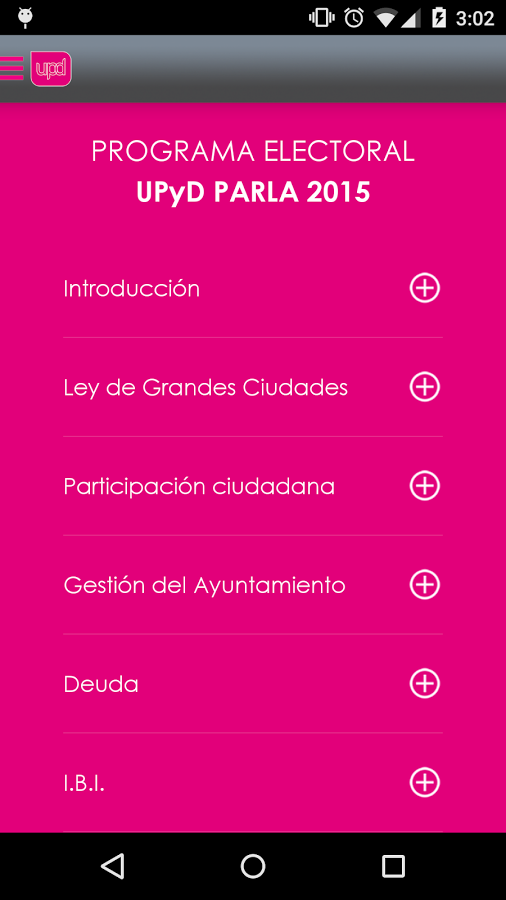
\includegraphics[keepaspectratio, scale=0.35]{Media/Captures/UPyDParla.png}
\caption{UPyD Parla}
\label{fig:upydparla}
\end{figure}

\subsubsection{$\sharp$RecuperaCórdoba}
De forma similar a la anterior, la candidatura de Pedro García a la provincia de Córdoba de Izquierda Unida, presenta su propuesta de gobierno de forma compacta. En la aplicación podremos encontrar la lista de los candidatos propuestos a la comunidad cordobesa, el programa electoral de la formación, las propuestas del partido, noticias de última hora y vídeos.

\begin{figure}[H]
\centering
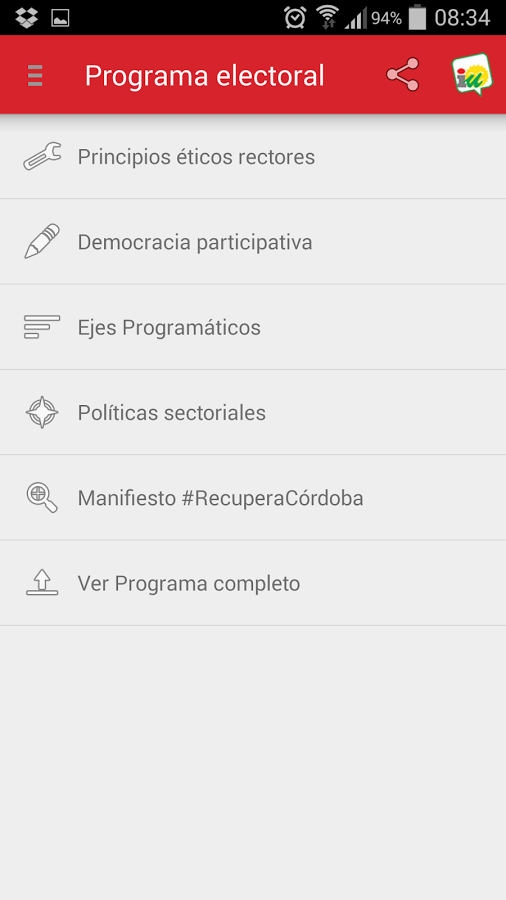
\includegraphics[keepaspectratio, scale=0.35]{Media/Captures/IURecuperaCordoba.png}
\caption{$\sharp$RecuperaCórdoba}
\label{fig:recuperacordoba}
\end{figure}

\subsubsection{PP Canarias}

La delegación del Partido Popular en Canarias, presenta su aplicación móvil para promocionar a sus candidatos para las elecciones autonómicas y municipales de Mayo de 2015. La aplicación nos avisará de los eventos electorales, podremos consultar los candidatos, novedades, galería de imágenes y por su puesto el programa electoral.

\begin{figure}[H]
\centering
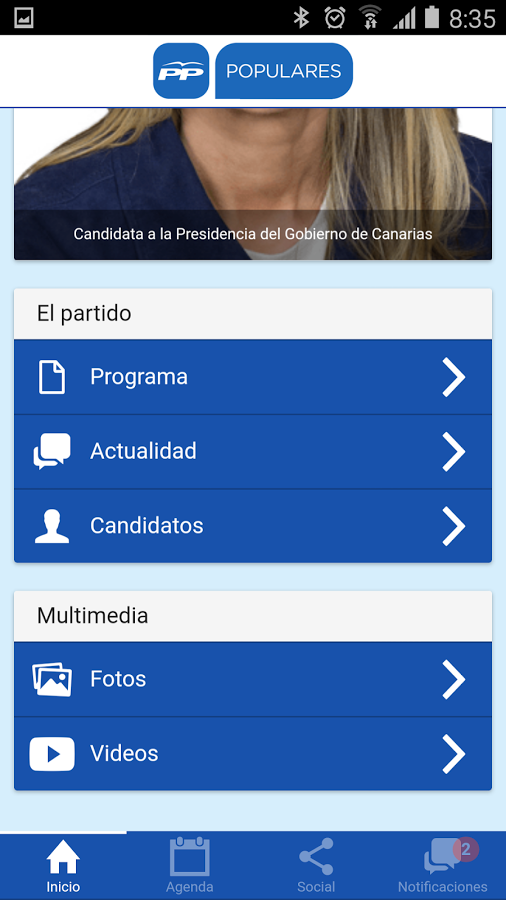
\includegraphics[keepaspectratio, scale=0.35]{Media/Captures/ppcanarias.png}
\caption{PP Canarias}
\label{fig:ppcanarias}
\end{figure}

\subsection{Participación Ciudadana}

Centrándonos en la participación ciudadana ya sea generación de propuestas, desarrollo colaborativo de programas o recogida de firmas, existen numerosos portales en internet y aplicaciones móviles destinadas a ello. Realizaremos un breve repaso a las aplicaciones más destacadas.

\subsubsection{reddit}

Reddit \cite{ref:reddit} es un sitio web donde los usuarios pueden crear temas, propuestas o compartir enlaces web a otros sitios. A primera vista puede parecer un foro, la principal diferencia respecto a este último radica en que oros usuarios pueden votar a favor o en contra de los enlaces, haciendo que aparezcan más o menos destacados. De tal forma que los temas de conversación, enlaces, o propuestas aparecerán en el orden que haya escogido la comunidad según la puntuación positiva o negativa.
En principio el uso de reddit está destinado a todos los temas, donde podemos encontrar algunos ejemplos relacionados fuertemente con la participación ciudadana en Plaza Podemos \cite{ref:plazaPodemos}. Un espacio utilizado para que la ciudadanía pueda expresar sus propuestas, compartir noticias relacionadas con la actualidad política o debatir aquellos temas que más preocupan. Así de un simple vistazo podemos saber qué es lo más debatido entre la ciudadanía, las propuestas que quieren llevar a cabo en en el gobierno o cuales son los temas que más preocupan.

\begin{figure}[H]
\centering
\includegraphics[keepaspectratio, scale=0.35]{Media/Captures/plazaPodemos.png}
\caption{Plaza Podemos utilizando reddit}
\label{fig:plazaPodemos}
\end{figure}

\subsubsection{Change.org}

Change.org \cite{ref:changeOrg} es portal web que permite alojar múltiples peticiones por internet. Podríamos definirlo como la evolución de la recogida de firmas en la calle. Cualquiera puede realizar una petición para solicitar apoyos. Las personas que decidan apoyar la petición, dejarán sus datos personales y constarán entre un número de personas que han apoyado la petición. Una vez que han alcanzado un número se procede a entregar las firmas digitales al organismo, persona o entidad a la que va destinada la petición.

En mayo de 2011, en relación con las movilizaciones del Movimiento 15-M y Democracia Real Ya, ante el desalojo por los Mozos de Escuadra se llevó a cabo la petición “Exige la dimisión fulminante del Conseller de Interior Felip Puig por la violencia utilizada en Pza. Catalunya”.

Desde su creación en 2007, change.org ha logrado muchas de sus peticiones demandadas entre los que se incluyen la atención de pacientes con enfermedades complejas, protección sobre animales y medio ambiente, derechos públicos, leyes, etcétera.

\begin{figure}[H]
\centering
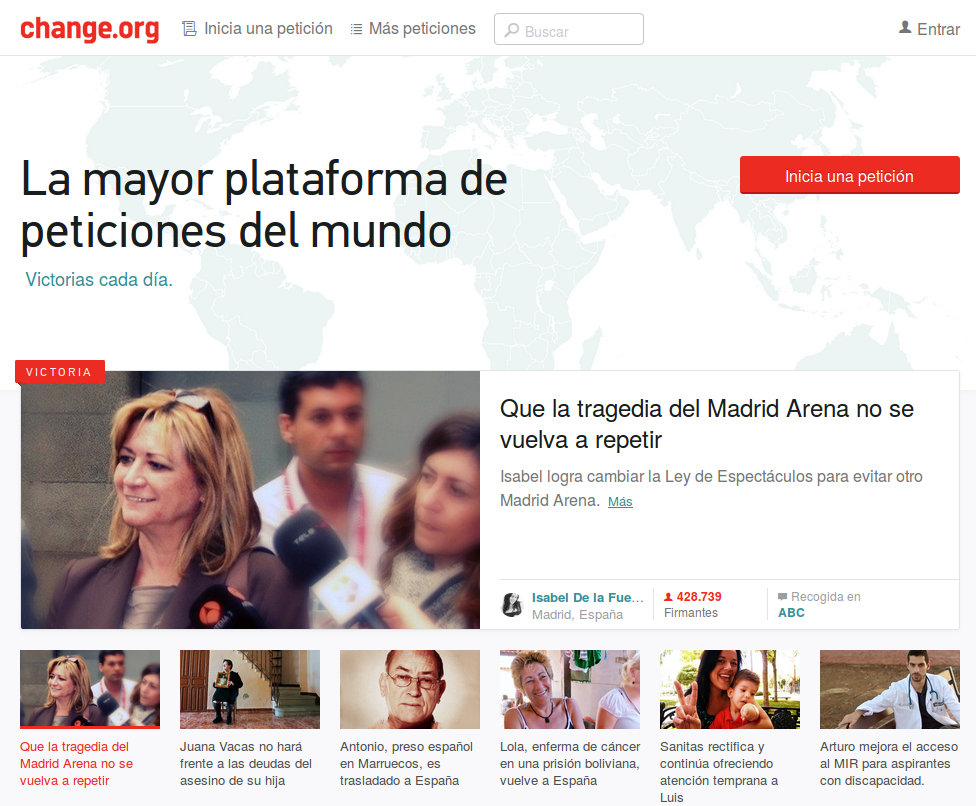
\includegraphics[keepaspectratio, scale=0.35]{Media/Captures/changeOrg.png}
\caption{Change.org · La mayor plataforma de peticiones del mundo}
\label{fig:changeOrg}
\end{figure}

\subsubsection{Programa Colaborativo AhoraMadrid}

Para las pasadas elecciones municipales del 24 de Mayo, la candidatura de unidad popular Ahora Madrid, desarrolló una plataforma en la web para elaborar su programa electoral de forma colaborativa. En esta plataforma, cualquier usuario tenía la oportunidad de explorar las propuestas por categoría o por distrito. De tal forma que podría debatirlas, puntuarlas o crear sus propias propuestas. Así las propuestas más valoradas por la comunidad, serían llevadas al programa final para las elecciones municipales del 24 de Mayo.

\begin{figure}[H]
\centering
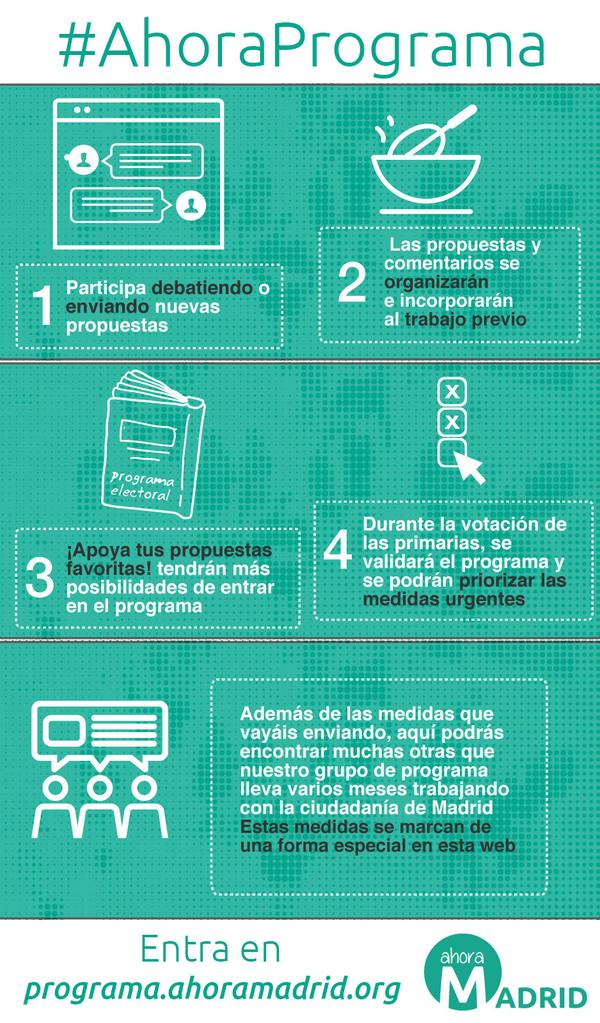
\includegraphics[keepaspectratio, scale=0.35]{Media/Captures/programaAhoraMadrid.jpg}
\caption{Creación colaborativa del programa de Ahora Madrid.}
\label{fig:programaAhoraMadrid}
\end{figure}